\documentclass{article} % For LaTeX2e
\usepackage{nips15submit_e,times}
\usepackage{hyperref}
\usepackage{url}
%\documentstyle[nips14submit_09,times,art10]{article} % For LaTeX 2.09
\usepackage[pdftex]{graphicx}  % omogoča vlaganje slik različnih 
\usepackage{wrapfig}
\usepackage{caption}
\usepackage{subcaption}
\usepackage{listings}
\usepackage{natbib}
\usepackage{todo}
\newtheorem{theorem}{Theorem}[section]
\usepackage{amsmath}
\usepackage[]{algorithm2e}






\title{Neural network pruning with simultaneous matrix tri-factorization and non-negative matrix factorization}
\author{Teja Ro\v{s}tan}
%\template is for anonymous submission

% The \author macro works with any number of authors. There are two commands
% used to separate the names and addresses of multiple authors: \And and \AND.
%
% Using \And between authors leaves it to \LaTeX{} to determine where to break
% the lines. Using \AND forces a linebreak at that point. So, if \LaTeX{}
% puts 3 of 4 authors names on the first line, and the last on the second
% line, try using \AND instead of \And before the third author name.

\newcommand{\fix}{\marginpar{FIX}}
\newcommand{\new}{\marginpar{NEW}}

\nipsfinalcopy % Uncomment for camera-ready version

\begin{document}


\maketitle

\begin{abstract}

In this paper we present the Matrix Factorization-based Brain Pruning (MFBP) method for 
pruning neural networks. MFBP finds and prunes redundant connections by mapping connection
weight matrices into a low-dimensional space. Simultaneous matrix tri-factorization is 
used to prune fully connected layers, and non-negative matrix factorization is used 
to prune the convolutional layers. We evaluated the MFBP method on two data sets. There, 
the reduced neural networks maintained their generalization performance, while requiring 
less computation.

\end{abstract}

\section{Introduction}

Deep neural networks (DNN) are a popular approach to machine learning that is being used 
to solve widely different and complex problems, such as image, sound and text recognition.
However, they are computationally intensive to train and yield black-box models that are 
difficult to interpret. Success of neural networks largely depends on their architecture. 
While the size of the input layer and the output layer is given in advance, the number and
size of hidden layers depends on the complexity of the problem~\cite{augasta2013pruning}. 

Generally, a network with large number of hidden nodes is able to learn fast and avoids
local minima, but an oversized network may overfit the training data and lose its 
generalization ability. Smaller networks are preferred because they usually achieve good 
generalization performance and are easier to interpret. Networks that are too small may be
sensitive to initial conditions, choice of learning parameters and usually do not 
generalize well. The most popular approach to obtain the optimal architecture of a DNN is 
to start with a slightly larger DNN and then apply pruning. Pruning algorithms remove the 
redundant connections while maintaining and sometimes improving the network generalization
performance~\cite{augasta2013pruning}.

Modern DNN can be extremely large, evolving many hidden layers with millions of parameters
and requiring large computation and storage cost. This prohibits their usage on resource 
limited mobile or embedded devices, which are most suited for applications involving 
DNNs~\cite{DBLP:journals/corr/GongLYB14}.

In this work we present a novel approach to pruning, named matrix factorization-based 
brain pruning (MFBP). The method is based on low-dimensional matrix factorization and is 
able to consider the entire structure of a neural network when pruning individual parts of
the network. The method uses simultaneous matrix tri-factorization to prune the fully 
connected layers, and non-negative matrix factorization (NMF) to prune the convolutional 
layers.

Source code for the MFBP method and code for the supporting experiments is available
at \url{https://github.com/teja-rostan/mfbp}.

\section{Related work}

Because there is significant redundancy in the parametrization of networks, many 
researchers proposed solutions to prune DNNs where initial extensive pruning is followed 
by backpropagation to fine-tune the pruned network and restore its generalization 
performance.

In convolutional neural network (CNN), about 90\% of the model size is taken up by the 
fully connected layers and more than 90\%  of the running time is taken by the 
convolutional layers~\cite{zeiler2014visualizing}. Compressing the most storage demanding 
fully connected layers is possible by pruning with low-rank matrix factorization (MF)
methods~\cite{lecun1989optimal, hassibi1993optimal, bondarenko2014artificial, 
sainath2013low}. Optimal Brain Damage (OBD)~\cite{lecun1989optimal} and Optimal 
Brain Surgeon (OBS)~\cite{hassibi1993optimal} are state-of-the-art approaches where OBS 
is one of the best methods for pruning. Likewise OBD, it should hold the Hessian matrix, 
thus requiring additional memory. Because the last fully connected layer is most 
parametrized, by pruning only last layer we can gain 30-50\% model size 
reduction~\cite{sainath2013low}. Method proposed by 
\textit{Bondarenko}~\cite{bondarenko2014artificial} can significantly simplify networks 
but it is not applicable on larger data sets and bigger models. Alternative 
approach~\cite{xue2013restructuring} uses a singular value decomposition (SVD) as low-rank
MF to reconstruct the weight matrices of the fully connected layers, reducing model size 
for 80\% and because of fine-tuning, with negligible accuracy loss. Opposite to our 
approach, they did not focus on convolutional layers to reduce testing time.

Low-rank MF can also be used to reduce time complexity~\cite{zhang2015efficient}.  
In~\cite{jaderberg2014speeding} CNN kernel maps were approximated with a low rank basis of
kernels that are separable in the spatial domain and drastically speedup computations.
Alternatively, each convolutional and fully connected layer can be compressed by finding 
an appropriate low-rank approximation with considering several elementary tensor 
decompositions based on SVDs~\cite{denton2014exploiting}. Both methods were successful at 
reducing model size by compressing to 90\% with negligible loss, meanwhile compressing 
convolutional layers up to 50\%.

Beside DNN pruning with MF many alternatives have been used in numerous ways to reduce 
model size. One of the latest studies~\cite{DBLP:journals/corr/GongLYB14} used strong 
vector quantization methods. A simple solution uses a constant number of simpler neurons 
with sparsity-inducing regularizers, which was presented in 
article~\cite{collins2014memory}. Another method uses the significance of neurons by  
evaluating the information on weight variation and consequently prune the insignificant
nodes on fully connected and on convolutional layers~\cite{han2015learning}. There, the 
first phase learns which connections are important and removes the unimportant ones using 
multiple iterations. They were also more successful at compressing fully connected layers
comparing to convolutional layers. Because iterative pruning dramatically increased 
pruning performance~\cite{han2015learning}, we also introduced iterative pruning in 
convolutional layers.

In article~\cite{anwar2015structured} they proposed to reduce time complexity with 
structured pruning and fixed point optimization. This work is the most similar to ours, as
they prune by changing redundant weight values to zero. They introduced structured 
sparsity at various scales for CNN. With channel pruning all weights to a feature map may 
be pruned. With kernel pruning full kernels can be dropped. Intra-kernel pruning prunes 
specific weights within a kernel~\cite{anwar2015structured}. In our work, we focus in 
intra-kernel pruning.

Dropout~\cite{srivastava2014dropout} and Dropconnect~\cite{wan2013regularization} randomly
zeroes neuron outputs and weights only during training for generalization purposes
and the network architecture does not change at evaluation time. Our work drops parameters
permanently, therefore, yields network with fewer parameters at test time.

%\todo{Many "similar" methods to ours exist. We do not show empirically how our 
%method compares to other. This is a major deficiency of our paper.}

\section{Approximation of weights in neural network}
\begin{figure}[!ht]
\centering
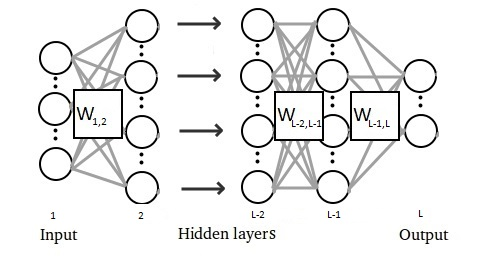
\includegraphics[width=.65\linewidth]{DNN2.jpg}
\captionof{figure}{Deep neural network with fully connected layers. Relation
matrix $W_{i,j}$ stores the weights of connections between neurons at layer $i$
and $j$.}
\label{f:dnn}
\end{figure}

Matrix factorization (MF) is a technique to  approximate the data in low-dimensional space
and to find latent features, which are a linear representation of data.

With ordinary artificial neural network, when there is only one hidden layer, the two 
weight matrices share the same dimension. In such cases, the two matrices can be 
concatenated and MF can be applied. Deep neural networks~\ref{f:dnn} have a multi-layer 
architecture where only neighbour weight matrices share the same dimension. We can 
directly apply co-dependency between two neighbouring weight matrices, but we can not 
apply dependency between, for example, between the first and third weight matrix. Our goal
is to consider the entire structure of a DNN, including relations between layers that are 
not connected directly.


\subsection{Approximation of weights in fully connected layers}

We use simultaneous matrix tri-factorization for pruning in fully connected layers. The 
theorem of simultaneous matrix tri-factorization states that all available relation 
matrices $W_{ij}$ can be simultaneously factorized into $G_i \in \Re^{m \times 
k}$, $G_j \in \Re^{n \times h}$ and $S_{ij} \in \Re^{k \times h}$. The factorization can 
be regularized through constrain matrices $\theta_i$ and $\theta_j$, such that $W_{ij} 
\approx G_iS_{ij}G_j^T$~\cite{zitnik2015data}~\ref{f:mf2}.

\begin{figure}[!ht]
\centering 
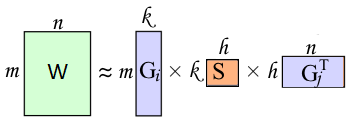
\includegraphics[width=.5\textwidth]{mf2.png}
\caption{Graphical visualization of simultaneous matrix tri-factorization.}
\label{f:mf2}
\end{figure}

Figure~\ref{f:dnn} shows a neural network with hidden layers and their relation weight 
matrices $W_{ij}$ between layers. The weight matrices can be placed into a grid, i.e., 
into a matrix of relations $W$, as shown in equation~\ref{eq:1}. A block in the $i$-th row
and $j$-th  column ($W_{ij}$) of matrix $W$ represents the relationship between object 
type $\xi_i$  and $\xi_j$. In case of a DNN, these represent neurons at layers $i$ and 
$j$, respectively. The block matrix $W$ is tri-factorized into block matrix factors $G$ 
and $S$. A factorization rank $k_i$ is assigned to $\xi_i$ during inference of the 
factorized system. Factors $S_{ij}$ define the relations between layers $\xi_i$ and 
$\xi_j$, while factors $G_i$ are specific to layers $\xi_i$ and are used in the 
reconstruction of every relation with this layer. In this way, each weight matrix $W_{ij}$
obtains its own factorization $G_i S_{ij} {G_j}^T$ with factor $G_i$ ($G_j$) that is 
shared across relations that involve layers $\xi_i$ ($\xi_j$). The objective function 
used for tri-factorization, as proposed by~\cite{zitnik2015data}, ensures good 
approximation of the weight matrices.

\begin{equation} \label{eq:1}
W = 
\begin{bmatrix} 
\begin{smallmatrix}
& &W_{1,2} & & & \\
& & &\ddots & & \\ 
& & & &W_{L-2,L-1} & \\ 
& & & & &W_{L-1,L} 
\end{smallmatrix}
\end{bmatrix} 
\approx 
\begin{bmatrix} 
\begin{smallmatrix}
& &G_1S_{1,2}G_2^T & & & \\ 
& & &\ddots & & \\ 
& & & &G_{L-2}S_{L-2,L-1}G_{L-1}^T & \\ 
& & & & &G_{L-1}S_{L-1,L}G_L^T 
\end{smallmatrix}
\end{bmatrix}
\end{equation}


We can reduce the number of neurons (parameters) in network as long as the number 
of parameters in $G_i$ and $G_j$ is less than the number of parameters in 
$W_{ij}$. To reduce the number of parameters in $W$ by a fraction of 
$p$~\cite{sainath2013low}, a selection of ranks $k_i$ must be made so that the 
equation~\ref{eq:2} holds.

\begin{equation} \label{eq:2}
 m_1k_1 + k_1h_2 + h_2n_2 + ... + m_{L-1}k_{L-1} + k_{L-1}h_L + h_Ln_L < 
p(m_1n_2 + ... + m_{L-1}n_L)
\end{equation}


\subsection{Approximation of weights in convolutional layers}

For convolutional layers we used a different approach. The kernel weights in different 
layers are usually independent. They share feature maps with their dimensions dependent 
from each input image. Because of this property, we have not found a solution based on MF 
that considers all connections that exist in all layers concurrently. We focused on every 
convolutional layer separately.

We used a non-negative matrix factorization (NMF) method for approximation. NMF is a 
recent method for finding such a representation~\cite{hoyer2004non}. Given a non-negative 
data matrix $W$ (kernel), NMF finds an approximate factorization $W \approx UV$ into 
non-negative factors $U$ and $V$. The non-negativity constraints make the representation 
purely additive (allowing no subtractions). 
We used two approaches:
\begin{itemize}
\item In every layer we approximated every kernel separately with NMF. 
\item In every layer we reshaped kernels to column vectors and concatenated them into a 
matrix, which we used for approximation with NMF (used in pseudocode~\ref{alg:MFBP}).
\end{itemize} Because the kernels in network are not constrained to non-negative 
values, we used the NMF method from Nimfa library~\citep{Zitnik2012}, which with 
preprocessing handles negative values in input matrix.


\section{Factorization-based brain pruning (MFBP)}

Candidates for pruning are those weights that when approximated move towards zero for a 
specified threshold, as given by the following formula:

$(abs(originalWeight) - abs(approximatedWeight)) >= threshold$

The threshold is set to user-specified percentile of all observed differences. Pruned 
weights are set to zero. The pruning procedure is defined in Algorithm~\ref{alg:MFBP}.
The code of MFBP is available on-line~\cite{code}.
\begin{algorithm}[H]
\label{alg:MFBP}
 \KwData{weight matrices $W$ of learned neural network, degree of pruning $p$}
 \KwResult{pruned weight matrices $Wp$}
 \For{every convolutional layer}{
   reshape kernels to column vectors\;
   concatenate kernels into a matrix $W_i$\;
   $A_i$ := approximation of $W_i$ with NMF\;
 }
 \For{every weight matrix $W_i$ in fully connected layers}{
  make relations\;
  add to relations graph $R$\;
 }
 apply simultaneous matrix tri-factorization on relations graph $R$\;
 \For{every weight matrix $W$ in relations graph $R$}{
  $A_i$ := approximations of $W_i$\;
 }
 $diff\_matrix$ := absolute($W$) - absolute($A$)\;
 $threshold$ = percentile $p$ of $diff\_matrix$\;
 \For{every approximated weight matrix $A$}{
  $Wp_i = W_i * (diff\_matrix_i \leq threshold)$\;
 }
 \caption{Pruning neural network with matrix factorization.}
 
\end{algorithm}

\section{Experimental setup}

We evaluated MFBP on MNIST~\cite{lecun-mnisthandwrittendigit-2010} and 
Cifar-10~\cite{krizhevsky2009learning} data sets. 

We pruned the neural network available at github~\cite{github}. The network inclused the 
ReLU (Rectified linear unit) activation function. It regularizes the network model with 
Dropout~\cite{srivastava2014dropout}. Instead of a standard stochastic gradient descent 
(SGD) backpropagation method, the network uses a RMSprop~\cite{lecture}. 

To evaluate our experiments, we implemented MFBP in Python, using the Theano 
library~\cite{Bastien-Theano-2012, bergstra+al:2010-scipy}, which offers great control 
over neural network formation. For simultaneous matrix tri-factorization, we used the data
fusion algorithm, which is  available in a python library 
Scikit-fusion~\cite{zitnik2015data}. For NMF we used the algorithm available in the Nimfa 
library~\cite{Zitnik2012}.


\section{Results}

We evaluated the predictive performance of the pruned networks with cross-validation. We 
used the Scikit-learn library~\cite{scikit-learn} to measure the area under ROC curve 
(AUC).


\subsection{Results on fully connected layers}

We trained six neural networks: three with two hidden layers (NN\_2HL) and three with four
hidden layers (NN\_4HL). Every neural network had 100 iterations available to learn. 
After learning, the simultaneous matrix tri-factorization was performed to prune weights. 
After pruning, 50 iterations of fine-tuning was used to refine the non-pruned weight 
values, which have been biased by the pruned weight. Every type of network had different 
amount of pruning. The reported results are measured on test set shown in 
figure~\ref{f:results}. 

\begin{figure}[!ht]
\centering
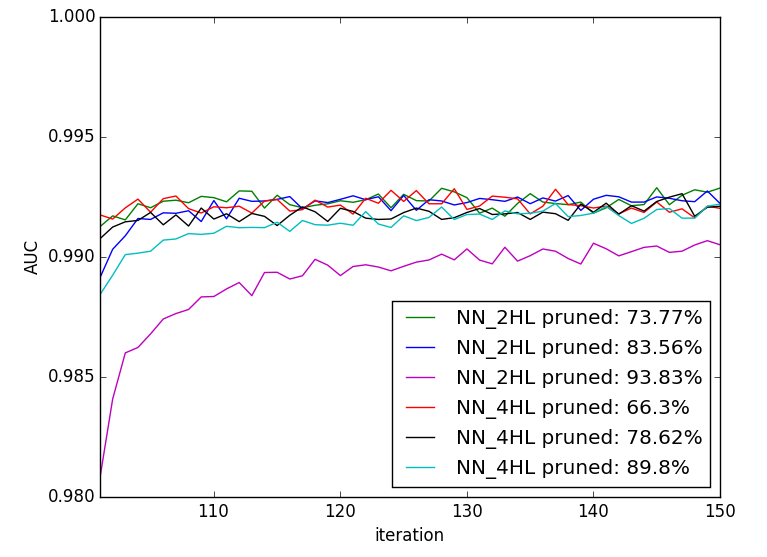
\includegraphics[width=0.8\linewidth]{nn.png}
\captionof{figure}{AUC results of six networks after pruning}
\label{f:results}
\end{figure}

We can observe that the networks with lower levels of pruning were able to recover the 
accuracy faster (after few iterations). In networks with higher amount of pruning, the 
non-pruned weights needed more iterations to recover to the accuracy from before pruning. 
Meanwhile, the network with two hidden layers, which was pruned the most (for 93,83~\%) 
was not able to recover as the amount of pruning was too high. From table~\ref{t:results} 
we can see that in most cases, the pruning resulted in slightly higher accuracy than 
before pruning, by pruning neural network up to 80\%. 


\begin{table}[!ht]
\centering
\begin{tabular}{l|l|l|p{3cm}|}
\cline{2-4}
 & max AUC score BP & max AUC score AP & a first AUC AP \textgreater= max AUC BP 
\\ \hline
\multicolumn{1}{|l|}{NN\_2HL pruned: 73.77\%} & 0.99272 at 72-iter & 0.99289 at 
145-iter & 0.99275 at 112-iter \\ \hline
\multicolumn{1}{|l|}{NN\_2HL pruned: 83.56\%} & 0.99291 at 88-iter & 0.99275 at 
149-iter & / \\ \hline
\multicolumn{1}{|l|}{NN\_2HL pruned: 93.83\%} & 0.99293 at 83-iter & 0.99068 at 
149-iter & / \\ \hline
\multicolumn{1}{|l|}{NN\_4HL pruned: 66.3\%} & 0.99236 at 97-iter & 0.99284 at 
129-iter & 0.99241 at 104-iter \\ \hline
\multicolumn{1}{|l|}{NN\_4HL pruned: 78.62\%} & 0.99236 at 78-iter & 0.99284 at 
147-iter & 0.99249 at 146-iter \\ \hline
\multicolumn{1}{|l|}{NN\_4HL pruned: 89.8\%} & 0.99201 at 99 iter & 0.99223 at 
137-iter & 0.99208 at 128-iter \\ \hline
\end{tabular}
\caption{AUC results from before pruning (BP) and after pruning (AP).}
\label{t:results}
\end{table}


\subsection{Results on convolutional layers}

We trained a network with three convolutional layers and one fully connected layer. 
Besides MNIST, we introduced the Cifar-10 data set. We used two previously mentioned 
approaches of kernel pruning with NMF. We also used multiple iterations of pruning, where 
the level of pruning increases with every pruning iteration. Iterations between pruning 
were reserved for recovering of weights that were kept. A recovering period lasted until 
five consecutive iterations where the network did not improve its performance.  

\begin{figure}[!ht]
\centering
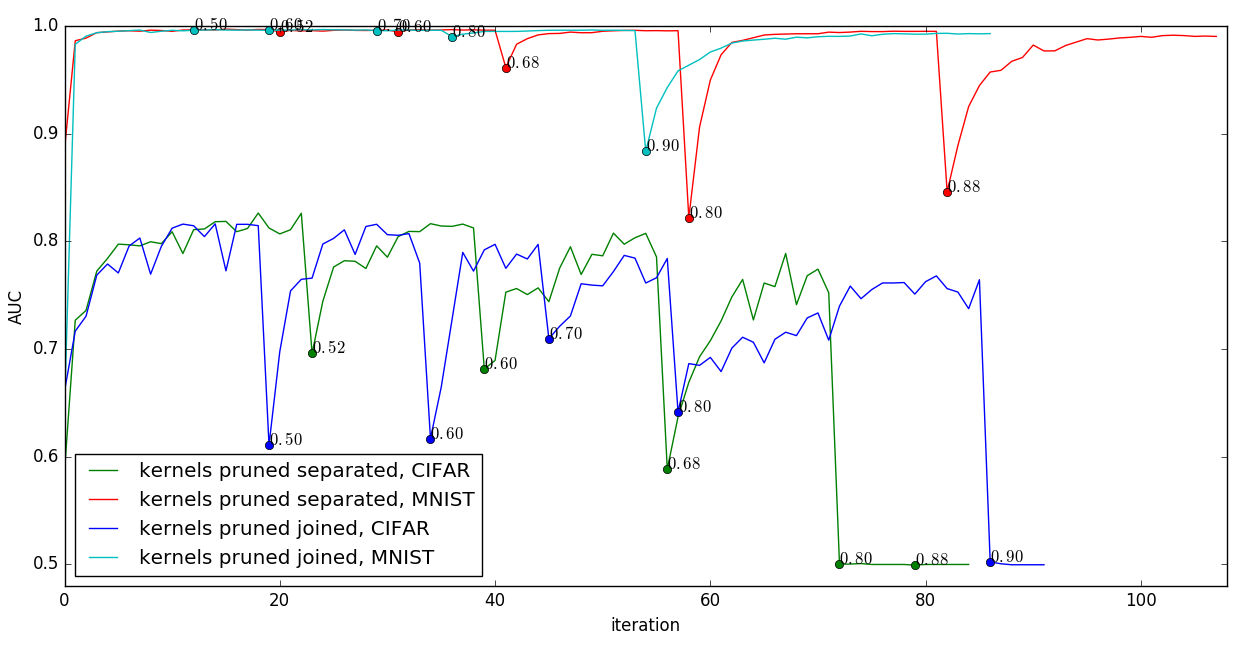
\includegraphics[width=1\linewidth]{auc_cnn.png}
\captionof{figure}{AUC results of two approaches on MNIST and CIFAR data set.}
\label{f:results_conv}
\end{figure}

\begin{figure}[!ht]
\centering
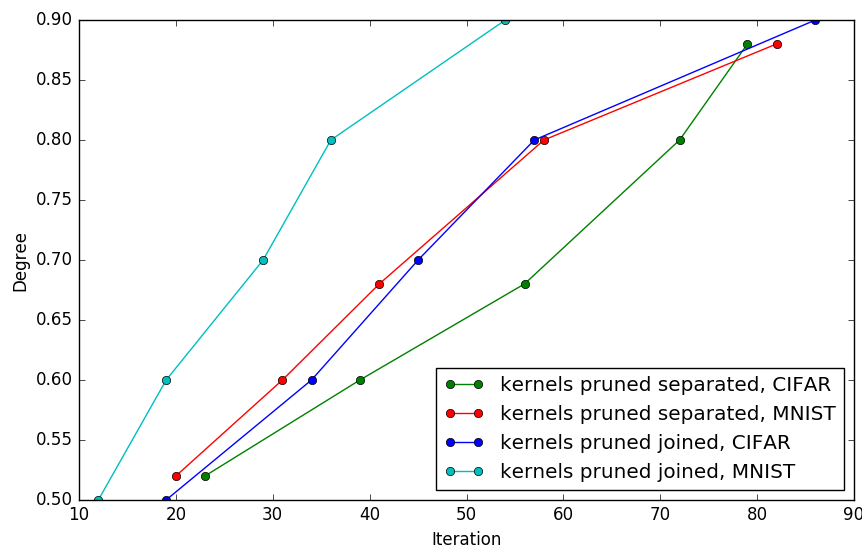
\includegraphics[width=.8\linewidth]{degree_cnn.png}
\captionof{figure}{Degree of pruning.}
\label{f:degree_conv}
\end{figure}

Figure~\ref{f:results_conv} show four AUC measures, for the two approaches and two
data sets. Pruning occurs at steps indicated by coloured dots and the associated number  
represent the degree of pruning at that step. Figure~\ref{f:degree_conv} shows the degree 
of pruning when pruning occurs.

From Figure~\ref{f:results_conv}, we can see that the pruned networks were able to 
recover lost accuracy to some degree. With stronger pruning, the recovery was less 
effective. When pruning by more than 80\% on the Cifar-10 data set, loss of all learned 
information occurred. The complete loss is related to the fact that the first 
convolutional layer has fewer parameters than the following layers. Because the first 
layer directly computes on the input data (layer), it is also more sensitive to 
pruning~\cite{anwar2015structured, han2015learning}. In our future, we should limit the 
level of pruning of the first layer, and pruning should be stopped at 80\%.

Overall, the proposed method \textit{kernels pruned joined}, which prunes concatenated 
kernel matrices at every layer, performed better than \textit{kernels pruned separated}, 
which prunes every kernel matrix separately. The \textit{kernels pruned joined} method is 
thus able to consider the similarities between kernels when pruning them.


\section{Discussion and conclusion}

In this paper, we have addressed size complexity of DNN by applying simultaneous matrix 
tri-factorization, which takes into account the entire structure of fully connected 
layers. We compressed network size considerably and with no loss in accuracy. We have 
addressed time complexity by applying NMF on kernels to speed up computations. We 
evaluated two methods for pruning kernels. One method prunes every kernel separately, 
while the other method concatenates kernels matrices from each layer into a matrix and 
prunes them simultaneously. The latter method performed better, as it can include 
similarities that exist between kernels in same layer. By pruning values in kernels we can
exploit its computational advantages~\cite{anwar2015structured}.

We did not compare our method with random pruning. Random pruning could be performed using
Dropout~\cite{srivastava2014dropout} and permanently dropping values to reduce model size 
and running time. This comparison is left for future work. The question on how to 
simultaneously and efficiently prune all the elements of a modern neural network, 
including input, convolutional, pooling, fully connected, and loss layers remains open.

%\subsubsection*{Acknowledgments}
%\subsubsection*{References}

\bibliographystyle{plain}
\bibliography{literature}

\todos

\end{document}








